

\item  (12 points)
    \begin{enumerate}
        \item (3 points) Complete the 5-by-5 magic square below so that every row, every column, and every diagonal have the same sum, and so that each integer from 1 through 25 is used exactly once.
        
        \renewcommand{\arraystretch}{2}%
\begin{tabular}{ | *{5}{>{\collectcell\fwcell}c<{\endcollectcell} |} }
  \hline
  {19} & {25} & 8 & 11 & {2}\\
  \hline
  {13} & {1} & 17 & 24 & 10 \\
  \hline
  22 & 9 & {15} & {3} & {16} \\
  \hline
  {5} & 18 & {21} & 7 & 14 \\
  \hline
  {6} & 12 & {4} & {20} & 23 \\
  \hline
\end{tabular}
\\
        \item (3 points) Give an expression for the column sum of an $n$-by-$n$ magic square.
        
        \hfill
                \begin{tabular}{|l|c|}
                    \hline
                    Answer for (\theenumii): & ${n(1+n^2)/2}$ \\ \hline
                \end{tabular}
                \\
        \item (3 points) Consider an arrangement of the positive integers, grouped as shown, so 
        that the $k$th group has $k$ elements: $(1),(2,3),(4,5,6),(7,8,9,10), \ldots$. Find 
        a formula for the sum of the $k$ numbers in the $k$th group.
        
        \hfill
                \begin{tabular}{|l|c|}
                    \hline
                    Answer for (\theenumii): & ${k(1+k^2)/2}$ \\ \hline
                \end{tabular}
                \\
        \item (3 points) Prove that your formula from the previous part is correct. 
        \hfill
        \\
        \\We define x as the mean of the set A, which has [1...$k^2$]. If we overlay k-th group numbers on A, we can conveniently notice that (observation 0) all the numbers in a k-th group belongs in set A in the same order, and centered inside A. I arbitrarily pick 3 and 4 as sample odd and even numbers to illustrate this property. 
        \\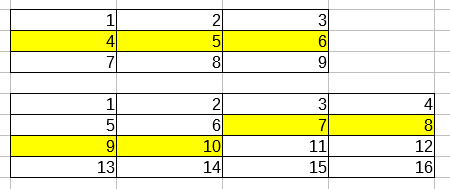
\includegraphics[]{5d.PNG}
        \\
        \\We can notice that (observation 1) if any pair of numbers is symmetric about a number, the mean of those two numbers is the original number. For example, 4 and 6 is symmetric about 5, since 4 is 1 less than 5 and 6 is 1 more than 5. This is the definition of central tendency. We also notice that (observation 2) a mean of any number is itself. For example, mean of 5 is 5. We also notice that (observation 3) if any number of sets has the same mean, the mean of the sum of the sets are the same as the individual means. For example, mean of (7,10) and mean of (8,9) is 8.5, same as mean of the individual sets.
        \\
        \\Therefore, in the case where k is even, we can pair the min and max of that set with each other, and pick the next min and the next max until all numbers are paired. Since all pairs are symmetric about the same center (due to the set being incremental by the same amount), we can say that all their mean are the same by observation 1. We can say that the mean of the set as a whole is the same as the individual means by observation 3. Because observation 0 (k-th number set is centered inside A) is true, we can say that their mean is the same as A's, defined as x, since we can apply the same pairing technique to A.
        \\
        \\The same pairing technique can be applied to cases where k is odd, by adding a pair of itself at the center of k-th numbers set and A numbers set. The mean of that pair is itself by observation 2, therefore not altering our conclusion from the even case.
        \\
        \\We can notice that 1 and $n^2$ are symmetric about x, therefore we can define x as the mean of 1 and $n^2$ by observation 1. To put that in math:
        \\$x = (1+k^2)/2$
        \\
        \\Since the mean is a number where the sum of residual (ie member - mean) is zero, we can say that the sum of any set is a multiple of its mean and its size. In other word:
        \\$x_1-\bar{x}+...+x_k-\bar{x} = 0$
        \\$x_1+...+\bar{x} = k\bar{x}$
        \\
        \\Therefore, we can say that sum of k-th group numbers set is the multiple of its mean, x, which is also defined as $(1+k^2)/2$. Therefore, we can conclude that:
        \\Sum of k-th group = $kx  = k(1+k^2)/2$
        \\
        \\\boxed{}
        \end{enumerate}
\vfill
        

\newpage
